\section{Ekstrakcja cech dźwiękowych}\label{rozdzial_ekstrakcja}
Cechami dźwiękowymi nazywamy zmienne wyekstrahowane z~sygnału audio, które opisują ten sygnał i~pozwalają uzyskać dodatkowe informacje na jego temat\cite{phdWork}. Opisane w~tym rozdziale zostały cechy sygnału audio, które są wejściami dla użytego klasyfikatora tj. sieci neuronowej. Poszczególne cechy bazowały zarówno na czasowej jak i~spektralnej reprezentacji sygnału.

\subsection{Cyfrowa reprezentacja sygnału audio}
Dźwięk jest sygnałem analogowym. W~celu przechowywania go na cyfrowych nośnikach spotkano się z~potrzebą jego digitalizacji tj. reprezentacji w~postaci cyfrowej. Najczęściej stosowaną w~tym celu jest metoda PCM\footnote{PCM - Pulse Code Modulation}
w~której to sygnał analogowy jest próbkowany w równych odstępach czasu i~zapisywany cyfrowo. Powszechnie stosowana częstotliwość próbkowania wynosi 44 100~Hz ze względu na zakres częstotliwości słyszanych przez człowieka, który wynosi około 20 000~Hz, a~zgodnie z~prawem Nyquista sygnał powinien być próbkowany z~dwa razy wyższą częstotliwością niż maksymalna częstotliwość sygnału w celu uzyskania dokładnej reprezentacji bez zniekształceń\cite{signalProcessing}. Przykładowy, reprezentowany cyfrowo, sygnał audio przedstawia rysunek \ref{audioExample1} oraz \ref{audioExample2}. Na rysunku \ref{audioExample2} przedstawiony został ten sam sygnał, który widzimy na rysunku \ref{audioExample1}, lecz w bardzo dużym przybliżeniu. Oba rysunki zostały wygenerowane za pomocą programu Audacity\cite{audacity} z~pliku audio w~formacie mp3\footnote{Format cyfrowego zapisu i~kompresji plików dźwiękowych}.

\begin{figure}[ht!]
\centering
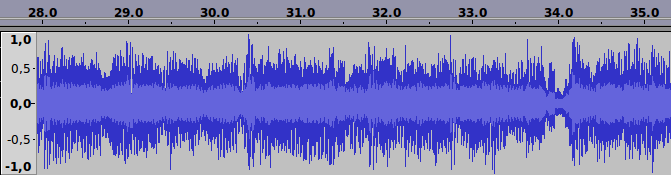
\includegraphics[scale=0.5]{res/exampleAudio1.png}
\caption{Przykładowy sygnał audio\label{audioExample1}}
\end{figure}

\begin{figure}[ht!]
\centering
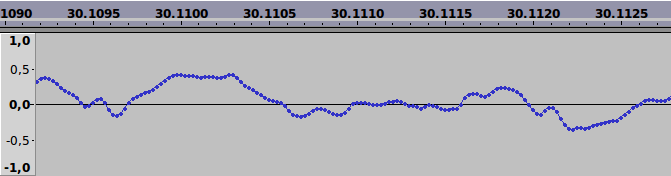
\includegraphics[scale=0.5]{res/exampleAudio2.png}
\caption{Przykładowy sygnał audio - przybliżenie\label{audioExample2}}
\end{figure}

\subsection{Spektralna reprezentacja sygnału audio}
\subsubsection{Transformacja Fouriera}
Każdy sygnał, który jest reprezentowany jako zmieniająca się w~czasie amplituda posiada też odpowiadające spektrum częstotliwościowe tzw. widmo. Dotyczy to także sygnału audio. Dzięki przedstawieniu sygnału dźwiękowego w~ten sposób możliwe jest uzyskanie dodatkowych informacji na jego temat\cite{windowingNI}. Spektrum przedstawia skład częstotliwościowy dźwięku. Przy obliczaniu spektrum z~pomocą przychodzi transformacja Fouriera. Oznaczając $x(t)$ jako sygnał, a~$X(f)$ jako wynik transformacji, możemy zapisać:
\begin{equation}
X(f)=\int\limits_{-\infty}^{\infty} x(t)e^{-j2\pi ft} dt ,
\end{equation}
przy czym $f$ to częstotliwość, natomiast $t$ oznacza czas. W~celu otrzymania spektrum amplitudowego, z~którego szeroko korzystano w~niniejszej pracy, należy z~otrzymanego wyniku obliczyć wartość bezwzględną:
\begin{equation}
|X(f)|.
\end{equation}
Trzeba jednak pamiętać, że w~przypadku sygnału audio zapisanego w~pamięci komputera mamy do czynienia z~sygnałem dyskretnym, więc należy użyć DFT\footnote{Discrete Fourier Transform} - transformaty Fouriera dla sygnałów dyskretnych wyrażającej się wzorem:
\begin{equation}
X_k = \sum_{n=0}^{N-1}x_n e^{-i2\pi\frac{k}{N}n} ,
\end{equation}
przy czym $x_n$ to kolejne wartości próbkowanego sygnału, $X_k$ to wartości transformaty. Na rysunku \ref{spectrumExample} przedstawiony jest przykładowy sygnał wraz z~odpowiadającym mu spektrum amplitudowym.

%https://en.wikipedia.org/wiki/Spectral_density#/media/File:Voice_waveform_and_spectrum.png
\begin{figure}[ht!]
\centering
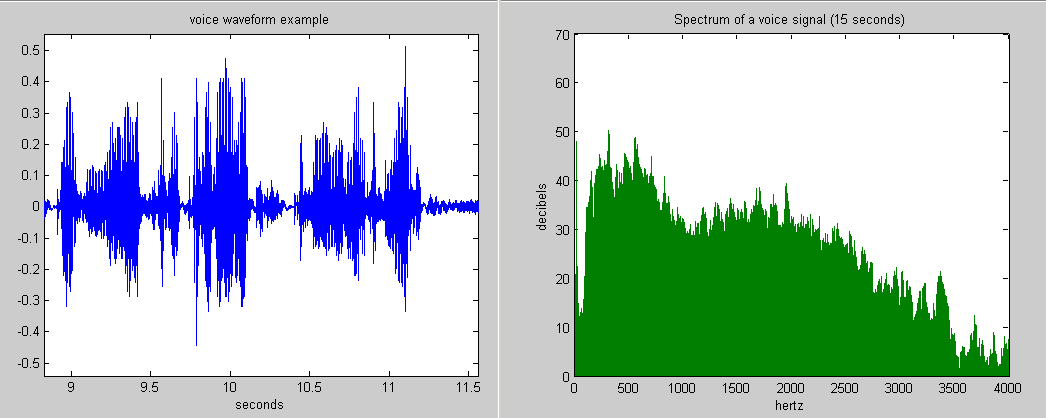
\includegraphics[scale=0.5]{res/spectrumExample.png}
\caption[Caption for LOF]{Sygnał audio wraz z odpowiadającym mu spektrum amplitudowym\label{spectrumExample} \footnotemark}
\end{figure}

\footnotetext{\url{https://commons.wikimedia.org/wiki/File:Voice_waveform_and_spectrum.png}}



\subsection{Wstępna obróbka sygnału}
Przed analizą sygnału dźwiękowego, jakim są utwory muzyczne, w~celu poprawy jakości danych przeprowadza się obróbkę wstępną, co pozwala na bardziej efektywną jego analizę. Przed ekstrakcją cech dźwiękowych wykorzystana została funkcja okna czasowego oraz algorytm wyrównywania poziomu głośności dźwięku opisane w~kolejnych dwóch podrozdziałach.

\subsubsection{Okno czasowe}
Ważną rolę przy korzystaniu z~transformaty Fouriera odgrywa okresowość. W~przypadku, gdy mamy do czynienia z~danymi, które występują niecałkowitą ilość razy, na końcach analizowanych danych występują nieciągłości, które powodują, że otrzymane spektrum jest zniekształcone. Rozwiązaniem tego problemu jest okno czasowe. Jest to funkcja, którą mnożymy przy sygnał w celu zmniejszenia zniekształceń\cite{windowingNI}. 

\subsubsection{Algorytm wyrównywania poziomu głośności dźwięku}
Ludzkie ucho nie słyszy dźwięków o~wszystkich częstotliwościach jako dźwięków o~tym samym poziomie głośności. Problem ten można rozwiązać częściowo przy użyciu algorytmu wyrównywania poziomu głośności, który filtruje dźwięk korzystając z~krzywych izofonicznych. Pojecie izofony lub też krzywej izofonicznej określa w fonach\footnote{Fon - jednostka poziomu głośności} słyszalne natężenie dźwięku w~zależności od częstotliwości\cite{izofona}. Ze względu na subiektywność postrzegania głośności nie istnieją ściśle określone krzywe izofoniczne. Istnieje jednak model zaproponowany przez Fletchera oraz Munsona\cite{izofonyModel}, który jest przedstawiony na rysunku \ref{izofony}.

%obrazek
% autor „FletcherMunson ELC” autorstwa Oarih - Created by Oarih using Inkscape. Licencja CC BY-SA 3.0 na podstawie Wikimedia Commons - https://commons.wikimedia.org/wiki/File:FletcherMunson_ELC.svg#/media/File:FletcherMunson_ELC.svg
\begin{figure}[ht!]
\centering
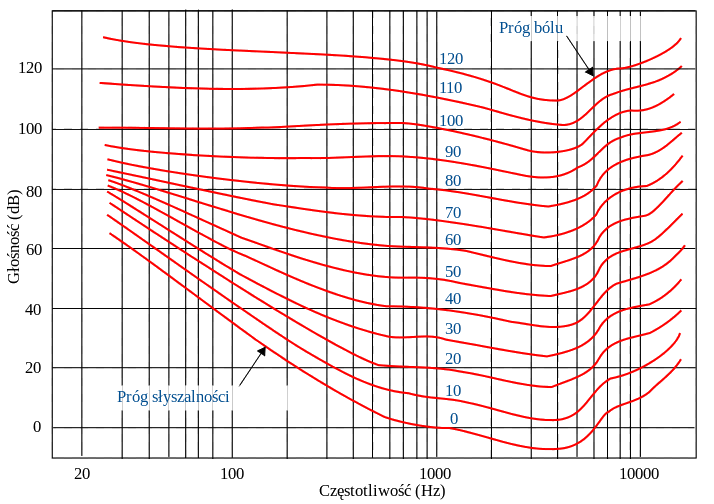
\includegraphics[scale=0.5]{res/equalLoudness.png}
\caption[Caption for LOF]{Izofony „normalnego” ucha według Fletchera i Munsona\footnotemark, wartości fonów dla poszczególnych krzywych określone są liczbami w kolorze niebieskim\label{izofony}
}
\end{figure}
\footnotetext{\url{https://commons.wikimedia.org/wiki/File:FletcherMunson_ELC.svg}}


\subsection{Cechy dźwięku bazujące na czasowej reprezentacji dźwięku}
W~niniejszym rozdziale zostały krótko opisane cechy dźwięku, które zostały rozważone w~pracy. W~kolejnych podrozdziałach oznaczono $f_i$ jako kolejne częstotliwości widma oraz $a_i$ jako odpowiadające im amplitudy.
\subsubsection{Wskaźnik zmiany znaku (\emph{Zero Crossing Rate})}
Wskaźnik zmiany znaku (\emph{Zero Crossing Rate}) jest jedną z~najprostszych cech dźwiękowych obliczanych z~wykorzystaniem reprezentacji dźwięku jako zmiana amplitudy w czasie. Wyraża on liczbę zmiany znaków w fali dźwiękowej w~jednostce czasu. Możemy określić go wzorem:
\begin{equation}
ZCR = \frac{1}{2} \sum^{N}_{n=1} |sgn(x[n]) - sgn(x[n-1])|.
\end{equation}
Jest to deskryptor często stosowany w~pozyskiwaniu informacji z~muzyki, ale także stosowany w~rozpoznawaniu mowy. Zawdzięcza to łatwości jego obliczania, a~także faktowi, że przechowuje informację o~szumach występujących w~dźwięku\cite{phdWork}.

\subsubsection{Wskaźnik zmian (\emph{Onset rate})}
Wskaźnik zmian (\emph{Onset rate}) jest podstawowym wskaźnikiem rytmu utworu muzycznego mającym duży wpływ na postrzeganie emocji reprezentowanych przez muzykę, ponieważ mówi o~zmienności dźwięku. Jest on określany jako liczba ekstremów obwiedni dźwięku\footnote{Krzywa opisująca zmianę amplitudy
sygnału\cite{obwiednia}}. Zakłada się, że różnica czasowa pomiędzy dwoma zmianami branym pod uwagę w~zliczaniu musi wynosić przynajmniej 60 ms\cite{phdWork}. 
 
\subsection{Cechy dźwięku bazujące na spektralnej reprezentacji dźwięku}
\subsubsection{Złożoność spektralna (\emph{Spectral complexity})}
Złożoność spektralna (\emph{spectral complexity}) jest liczbą ekstremów w~widmie amplitudowym sygnału dźwiękowego. Opisuje ona złożoność tego widma. Utwory z~większą średnią złożonością spektralną charakteryzują się większą energicznością\cite{phdWork}.

\subsubsection{Kształt spektralny (\emph{Spectral shape})}
Kształt spektralny jest kształtem widma amplitudowego danego sygnału dźwiękowego. W~jego skład wchodzą m.in. środek masy widma sygnału (\emph{spectral centroid}), współczynnik skośności widma sygnału (\emph{spectral skewness}), kurtoza widma sygnału (\emph{spectral kurtosis}), tzw. \emph{spectral roll-off} oraz rozrzut spektralny (\emph{spectral spread}). Wszystkie te cechy mają wpływ na odbiór utworu muzycznego przez słuchacza pod kątem reprezentowanych przez utwór emocji\cite{phdWork}.

\paragraph{Moment centralny}\mbox{}\\
W~celu określenia kolejnych wzorów mówiących o kształcie spektralnym użyteczne jest zdefiniowanie momentu centralnego. Dla zmiennej dyskretnej moment centralny jest przedstawia się wzorem:
\begin{equation}\label{momentCentralny}
\mu = \sum^{N}_{i=1} \frac{(f_i - \overline{f})^r}{N},
\end{equation}
gdzie $f_i$ są kolejnymi częstotliwościami występującymi w~widmie, $\overline{f}$ średnią częstotliwością, natomiast $N$ to liczba wszystkich częstotliwości. Moment centralny rzędu drugiego obliczamy korzystając ze wzoru \ref{momentCentralny}:
\begin{equation}
\sigma ^ 2 = \sum^{N}_{i=1} \frac{(f_i - \overline{f})^2}{N}
\end{equation}
i~nazywany wariancją. Pierwiastek kwadratowy z~wariancji $\sigma$ określany jest mianem odchylenia standardowego.

\paragraph{Środek masy widma}\mbox{}\\
Środek masy widma wyrażamy wzorem:
\begin{equation}
SC = \frac{\sum f_i a_i}{a_i},
\end{equation}
gdzie $f_i$ jest częstotliwością, natomiast $a_i$ amplitudą dla poszczególnych częstotliwości\cite{phdWork}.

\paragraph{Współczynnik skośności widma}\mbox{}\\
Współczynnik skośności mówi o~asymetryczności widma. W przypadku, gdy jest on mniejszy od zera, więcej danych znajduje się po lewej stronie widma, w przypadku, gdy jest on większy od zera, więcej danych znajduje się po prawej stronie widma. Określa się go wzorem:
\begin{equation}
\gamma = \frac{\mu _3 }{\sigma ^3}
\end{equation}

\paragraph{Kurtoza widma}\mbox{}\\
Kurtoza widma jest miarą jego spłaszczenia, wyraża się wzorem:
\begin{equation}
K = \frac{\mu _4 }{\sigma ^4}
\end{equation}

\paragraph{\emph{Roll-off} widma}\mbox{}\\
Cechą dźwięku określana mianem \emph{Roll-off}'u widma jest częstotliwość, która dzieli widmo sygnału na dwie części według ustalonego progu $T$, który zazwyczaj wynosi 0.95\cite{phdWork}. Omawiana cecha jest zdefiniowana wzorem\cite{rollOff}:
\begin{equation}
\sum_{i=1}^{R_t}f_i = T \sum_{i=1}^{N}f_i.
\end{equation}

\paragraph{Rozrzut spektralny}\mbox{}\\
Rozrzut spektralny jest miarą mówiącą o~szerokości widma sygnału, który wyraża się wzorem:
\begin{equation}
spectralSpread = \frac{\sum_{i}^{}(f_i - SC)^2 a_i}{\sum_{i}a_i} 
\end{equation}
Utwory muzyczne o większym rozrzucie spektralnym charakteryzują się większą energicznością. % cite?

\subsubsection{Płaskość spektralna \emph{(Spectral flatness)}}
Płaskość spektralna jest stosunkiem średniej arytmetycznej do średniej geometrycznej widma amplitudowego wyrażonym w decybelach:
\begin{equation}
spectralFlatness=10 log_{10} \frac{G}{A}
\end{equation}
przy czym $G$ jest średnią geometryczną:
\begin{equation}
G=\sqrt[n]{\prod_{i=1}^{N} a_i}
\end{equation}
oraz $A$ jest średnią arytmetyczną:
\begin{equation}
A=\frac{\sum_{i=1}^{N}a_i}{N}.
\end{equation}
Cecha ta określa jak bardzo spłaszczony jest wykres widma amplitudowego. Wraz ze wzrostem tego wskaźnika dźwięk bardziej przypomina szum. Wartość bliska 1 świadczy o występowaniu białego szumu\footnote{Szum akustyczny o prawie płaskim widmie}\cite{phdWork}.


\subsubsection{Dysonans (\emph{Dissonance})}
Dysonans jest deskryptorem dźwięku obliczanym na podstawie odstępów pomiędzy ekstremami widma amplitudowego. W~przypadku utworów muzycznych cechujących się mniejszym rozdźwiękiem obserwuje się większą równomierność tychże odstępów. Matematycznie dysonans można określić wzorem:
\begin{equation}
dissonance = \frac{1}{H}\sum_{h=1}^{H} a(h) - SE(h),
\end{equation}
gdzie $H$ jest liczbą ekstremów, $a(h)$ amplitudą dla danego ekstremum oraz $SE(h)$ amplitudą obwiedni spektrum dla częstotliwości $f(h)$\cite{phdWork}.

\subsubsection{Skala}
Skala muzyczna składa się z~dźwięków o~różnych częstotliwościach ułożonych według ustalonego schematu. Możemy wyróżnić dwie podstawowe skale: molową oraz durową. Powszechnie uznaje się, że utwory muzyczne bazujące na skali durowej mają radosne brzmienie, natomiast na skali molowej smutne brzmienie\cite{skala}. W~celu wyekstrahowania skali muzycznej utworu należy najpierw obliczyć jego HPCP\footnote{Harmonic Pitch Class Profile}, który obliczany jest na podstawie ekstremów widma amplitudowego według wzoru:
\begin{equation}
HPCP(n) = \sum^{N}_{i=1} w(n,f_i)a_i ^2,
\end{equation}
gdzie $a_i$ oraz $f_i$ są kolejno amplitudą oraz częstotliwością ekstremum, $N$ jest liczbą wszystkich ekstremów, $n$ kolejną wartością wektora HPCP, natomiast $w$ funkcją wagową określającą w jaki sposób poszczególne ekstremum wpływa na wartość $n$ wartości wektora HPCP. W celu określenia skali muzycznej obliczana jest korelacja pomiędzy wektorem HPCP, a odpowiednimi profilami dla obu skali\cite{hpcp}.










    
